% ==============================================================================
% Supplementary Materials - Nature Publication Standard
% Paper: A Calibrated Transcriptomic Atlas of Porcine Development
% ==============================================================================
% Following Nature's Supplementary Information formatting guidelines:
% - Sans-serif font (Helvetica)
% - Double line spacing
% - Figure legends with bold titles
% - One figure per page recommended
% ==============================================================================
\documentclass[11pt,letterpaper]{article}

% Page layout - Nature-compliant margins
\usepackage[
  top=2.5cm,
  bottom=2.5cm,
  left=2.5cm,
  right=2.5cm
]{geometry}

% Typography - Sans-serif (Helvetica) as required by Nature
\usepackage[T1]{fontenc}
\usepackage{helvet}
\renewcommand{\familydefault}{\sfdefault}

% Essential packages
\usepackage{graphicx}
\usepackage{booktabs}
\usepackage{multirow}
\usepackage{siunitx}
\usepackage{amsmath}
\usepackage{amssymb}
\usepackage[hidelinks]{hyperref}
\usepackage{setspace}
\usepackage{caption}
\usepackage{subcaption}
\usepackage{url}
\usepackage{xcolor}
\usepackage{float}

% Line spacing - Nature recommends double spacing for review
\doublespacing

% Caption formatting - Nature style with bold title
\captionsetup{
  font={sf,small},           % Sans-serif, small font
  labelfont={bf},            % Bold label (Supplementary Figure 1)
  labelsep=period,           % Period after label
  justification=justified,
  singlelinecheck=false,
  format=plain,
  skip=10pt
}

% Figure placement - allow figures to fill page
\renewcommand{\floatpagefraction}{0.7}
\renewcommand{\topfraction}{0.9}
\renewcommand{\bottomfraction}{0.9}
\renewcommand{\textfraction}{0.1}

% Set graphics path
\graphicspath{{figures/output/pdf/}{figures/main/}{figures/supplementary/}}

% Custom commands for Nature-style formatting
\newcommand{\figref}[1]{Supplementary Figure~\ref{#1}}
\newcommand{\tabref}[1]{Supplementary Table~\ref{#1}}

% Document metadata
\title{%
  \textbf{Supplementary Information}\\[1em]
  \large A Calibrated Transcriptomic Atlas of Porcine Development\\
  Reveals Conserved Molecular Programs with Humans%
}
\author{}
\date{}

% ==============================================================================
\begin{document}

\maketitle

\tableofcontents
\clearpage

% Include supplementary content
% ==============================================================================
% Supplementary Materials - Nature Publication Standard
% Paper: A Calibrated Transcriptomic Atlas of Porcine Development
% ==============================================================================
\documentclass[11pt,letterpaper]{article}

% Page layout - Nature-compliant margins
\usepackage[
  top=2.5cm,
  bottom=2.5cm,
  left=2.5cm,
  right=2.5cm
]{geometry}

% Typography - Sans-serif (Helvetica) as required by Nature
\usepackage[T1]{fontenc}
\usepackage{helvet}
\renewcommand{\familydefault}{\sfdefault}
\usepackage{microtype}  % Improved typography

% Essential packages
\usepackage{graphicx}
\usepackage{booktabs}
\usepackage{multirow}
\usepackage{siunitx}
\usepackage{amsmath}
\usepackage{amssymb}
\usepackage[hidelinks]{hyperref}
\usepackage{setspace}
\usepackage{caption}
\usepackage{subcaption}
\usepackage{url}
\usepackage{xcolor}
\usepackage{float}
\usepackage{fancyhdr}
\usepackage{titlesec}
\usepackage{tocloft}
\usepackage{enumitem}

% Define Nature blue color
\definecolor{NatureBlue}{RGB}{0, 51, 102}

% Line spacing - 1.5 for readability (Nature allows this for supplementary)
\onehalfspacing

% Header and footer styling
\pagestyle{fancy}
\fancyhf{}
\fancyhead[L]{\small\textcolor{gray}{Supplementary Information}}
\fancyhead[R]{\small\textcolor{gray}{Liu et al.}}
\fancyfoot[C]{\thepage}
\renewcommand{\headrulewidth}{0.4pt}
\renewcommand{\footrulewidth}{0pt}

% Caption formatting - Nature style with bold title
\DeclareCaptionLabelSeparator{bar}{ $|$ }
\captionsetup{
  font={sf,small},
  labelfont={bf},
  labelsep=bar,
  justification=justified,
  singlelinecheck=false,
  format=plain,
  skip=10pt
}

% Section formatting
\titleformat{\section}
  {\Large\bfseries\sffamily\color{NatureBlue}}
  {\thesection}{1em}{}
\titlespacing*{\section}{0pt}{20pt}{10pt}

% ToC formatting
\renewcommand{\cftsecfont}{\sffamily\bfseries}
\renewcommand{\cftsecpagefont}{\sffamily}
\renewcommand{\cftdotsep}{1}
\setlength{\cftbeforesecskip}{8pt}

% Figure placement
\renewcommand{\floatpagefraction}{0.7}
\renewcommand{\topfraction}{0.9}
\renewcommand{\bottomfraction}{0.9}
\renewcommand{\textfraction}{0.1}

% Set graphics path
\graphicspath{{figures/output/pdf/}{figures/main/}{figures/supplementary/}}

% Custom commands
\newcommand{\figref}[1]{Supplementary Figure~\ref{#1}}
\newcommand{\tabref}[1]{Supplementary Table~\ref{#1}}

% Hyperref setup
\hypersetup{
  colorlinks=true,
  linkcolor=NatureBlue,
  citecolor=NatureBlue,
  urlcolor=NatureBlue,
  pdftitle={Supplementary Information: A Calibrated Transcriptomic Atlas of Porcine Development},
  pdfauthor={Tianyuan Liu et al.}
}

% ==============================================================================
\begin{document}

% Title and Table of Contents on a single page
\thispagestyle{empty}
\begin{center}
  \vspace*{1cm}
  
  {\Large\textcolor{NatureBlue}{\textbf{SUPPLEMENTARY INFORMATION}}}
  
  \vspace{1cm}
  
  {\LARGE\bfseries A Calibrated Transcriptomic Atlas of\\[0.3em]
   Porcine Development Reveals Conserved\\[0.3em]
   Molecular Programs with Humans}
  
  \vspace{1cm}
  
  {\large Tianyuan Liu, Rujing Lei, Ilyas M. Khan, Peter Theobald}
  
  \vspace{1.5cm}
  
  \rule{0.6\textwidth}{0.5pt}
  
  \vspace{0.5cm}
  
  {\small This file contains:}
  
  \vspace{0.3cm}
  
  \begin{itemize}[leftmargin=3cm, itemsep=0.2cm]
    \item[\textbullet] Supplementary Figures S1--S3
    \item[\textbullet] Supplementary Tables S1--S3
  \end{itemize}
  
\end{center}

\vspace{1cm}

% Table of contents
\tableofcontents
\clearpage

% Reset page numbering
\setcounter{page}{1}

% ==============================================================================
% SUPPLEMENTARY FIGURES
% ==============================================================================
% Nature-style formatting:
% - Bold brief title for each figure/table
% - Concise descriptions (≤100 words per figure)
% - Panel labels in lowercase (a, b, c)
% ==============================================================================

\section*{Supplementary Figures}
\addcontentsline{toc}{section}{Supplementary Figures}

% ------------------------------------------------------------------------------
% Supplementary Figure 1: Cross-species sensitivity analysis
% ------------------------------------------------------------------------------
\begin{figure}[H]
  \centering
  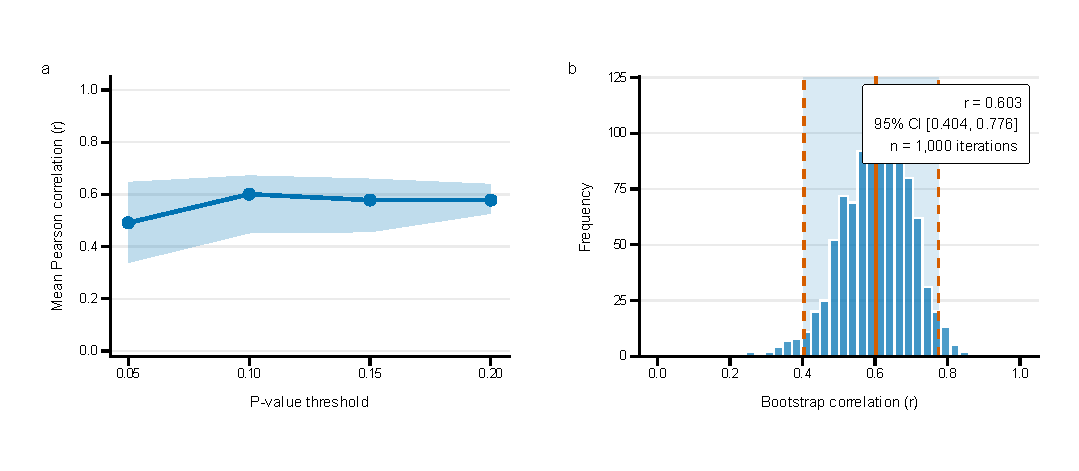
\includegraphics[width=\textwidth]{figures/output/pdf/figS1_cross_species_sensitivity.pdf}
  \caption{\textbf{Cross-species sensitivity analysis of conserved developmental markers.}
  \textbf{a}, Mean Pearson correlation between pig and human developmental fold changes across significance thresholds ranging from $p < 0.01$ to $p < 0.20$. Shaded region indicates the range (minimum--maximum) across different gene set sizes ($n = 15$--$50$ genes).
  \textbf{b}, Bootstrap distribution of correlation coefficients from 1,000 resampling iterations for the optimal parameter combination ($p < 0.10$, $n = 36$ genes). Solid vertical line indicates the observed correlation ($r = 0.62$); dashed lines denote the 95\% bootstrap confidence interval boundaries.}
  \label{fig:S1}
\end{figure}

\clearpage

% ------------------------------------------------------------------------------
% Supplementary Figure 2: Tissue specificity and feature stability
% ------------------------------------------------------------------------------
\begin{figure}[H]
  \centering
  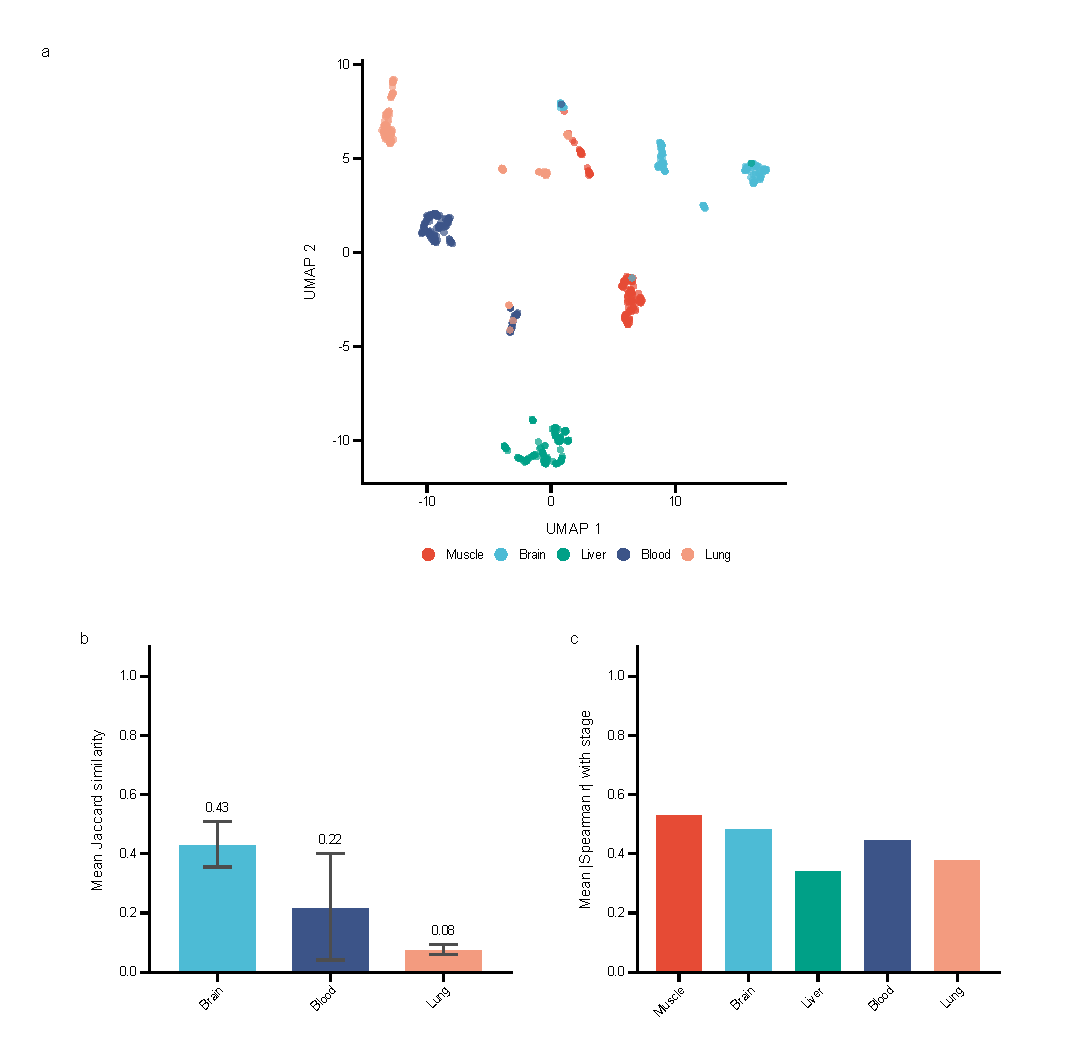
\includegraphics[width=\textwidth]{figures/output/pdf/figS2_tissue_specificity_stability.pdf}
  \caption{\textbf{Tissue specificity and feature selection stability analysis.}
  \textbf{a}, Uniform manifold approximation and projection (UMAP) of gene expression profiles across five tissues (muscle, brain, liver, blood, lung), demonstrating distinct tissue-specific clustering patterns ($n = 150$ samples per tissue, top 500 variable genes).
  \textbf{b}, Within-tissue feature selection stability quantified as mean Jaccard similarity index of the top 50 selected features across five independent random seeds. Error bars represent standard deviation; higher values indicate more reproducible feature selection.
  \textbf{c}, Mean absolute Spearman correlation of top-ranked features with developmental stage. Error bars represent standard deviation across selected features within each tissue.}
  \label{fig:S2}
\end{figure}

\clearpage

% ------------------------------------------------------------------------------
% Supplementary Figure 3: Extended performance metrics
% ------------------------------------------------------------------------------
\begin{figure}[H]
  \centering
  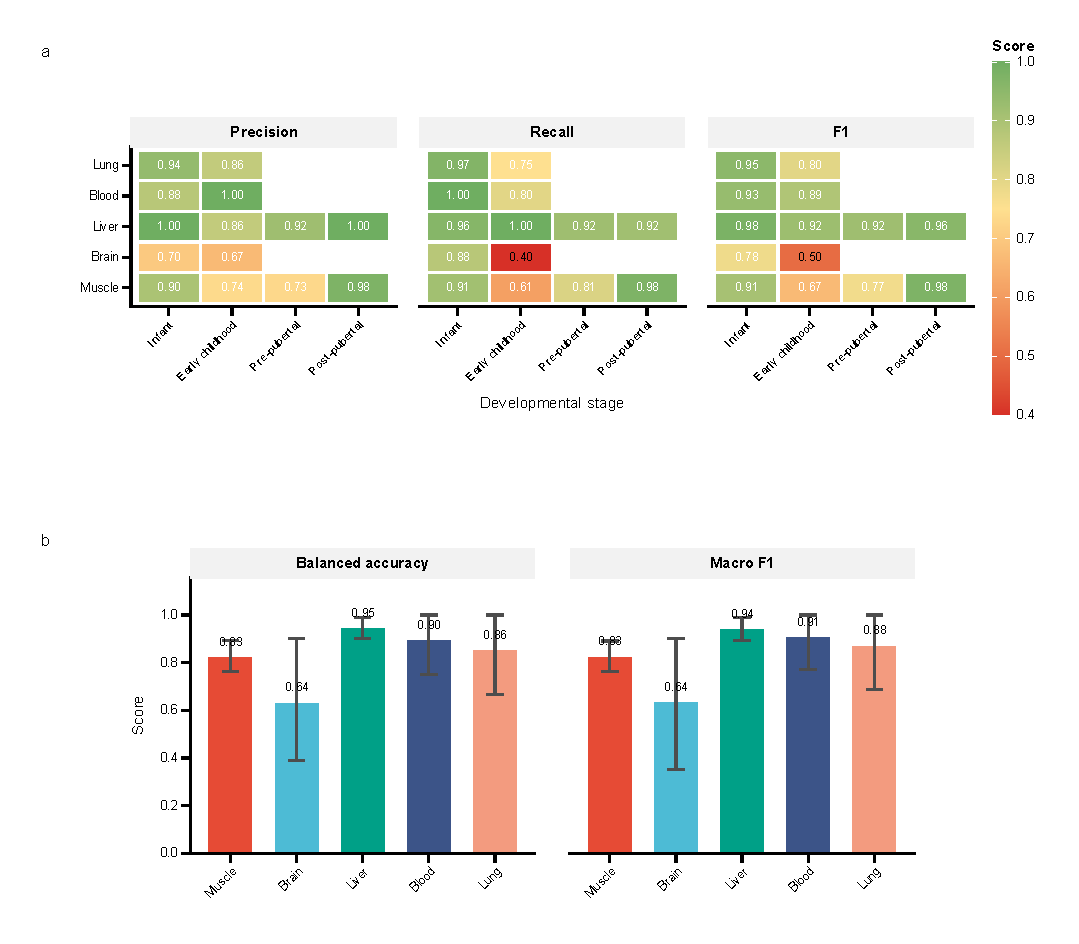
\includegraphics[width=\textwidth]{figures/output/pdf/figS3_extended_performance.pdf}
  \caption{\textbf{Extended classification performance metrics across tissues and developmental stages.}
  \textbf{a}, Heatmap of per-class precision, recall, and F1 scores for each developmental stage across all five tissues. Colour scale ranges from 0.4 (red, poor performance) to 1.0 (green, excellent performance). Missing values indicate developmental stages not present in that tissue's classification scheme.
  \textbf{b}, Overall performance summary showing balanced accuracy and macro-averaged F1 scores evaluated on the held-out test set (30\% of samples) for each tissue. Error bars indicate 95\% bootstrap confidence intervals from 1,000 resampling iterations.}
  \label{fig:S3}
\end{figure}

\clearpage

% ==============================================================================
% SUPPLEMENTARY TABLES
% ==============================================================================
\section*{Supplementary Tables}
\addcontentsline{toc}{section}{Supplementary Tables}

% ------------------------------------------------------------------------------
% Supplementary Table 1: Train vs Test Performance
% ------------------------------------------------------------------------------
\begin{table}[H]
  \centering
  \caption{\textbf{Train versus test performance comparison.} Test set performance (30\% held out) is reported for all tissues. Train set metrics are not shown as models were evaluated only on held-out data to prevent overfitting.}
  \label{tab:S1}
  \small
  \begin{tabular}{lcccccc}
    \toprule
    Tissue & Scheme & $n$ & Balanced Acc. & F1-macro & F1-weighted & MAE \\
    \midrule
    Muscle & 4-class & 761 & 0.844 & 0.842 & 0.908 & 0.10 \\
    Brain & 2-class & 43 & 0.637 & 0.639 & 0.671 & -- \\
    Liver & 4-class & 309 & 0.920 & 0.910 & 0.913 & 0.09 \\
    Blood & 2-class & 78 & 0.864 & 0.869 & 0.874 & -- \\
    Lung & 2-class & 129 & 0.859 & 0.876 & 0.921 & -- \\
    \bottomrule
  \end{tabular}
\end{table}

\vspace{2cm}

% ------------------------------------------------------------------------------
% Supplementary Table 2: Per-class performance
% ------------------------------------------------------------------------------
\begin{table}[H]
  \centering
  \caption{\textbf{Per-class performance metrics by tissue.} Precision, recall, and F1 scores for each developmental stage within each tissue. $n$ indicates the number of test samples per class.}
  \label{tab:S2}
  \small
  \begin{tabular}{llcccc}
    \toprule
    Tissue & Stage & $n$ & Precision & Recall & F1 \\
    \midrule
    Muscle & Infant & 58 & 0.912 & 0.897 & 0.904 \\
    Muscle & Early childhood & 23 & 0.714 & 0.652 & 0.682 \\
    Muscle & Pre-pubertal & 27 & 0.767 & 0.852 & 0.807 \\
    Muscle & Post-pubertal & 121 & 0.975 & 0.975 & 0.975 \\
    \midrule
    Brain & Infant & 8 & 0.700 & 0.875 & 0.778 \\
    Brain & Early childhood & 5 & 0.667 & 0.400 & 0.500 \\
    \midrule
    Liver & Infant & 26 & 1.000 & 0.962 & 0.980 \\
    Liver & Early childhood & 18 & 0.783 & 1.000 & 0.878 \\
    Liver & Pre-pubertal & 25 & 0.950 & 0.760 & 0.844 \\
    Liver & Post-pubertal & 24 & 0.920 & 0.958 & 0.939 \\
    \midrule
    Blood & Infant & 14 & 0.867 & 0.929 & 0.897 \\
    Blood & Early childhood & 10 & 0.889 & 0.800 & 0.842 \\
    \midrule
    Lung & Infant & 31 & 0.938 & 0.968 & 0.952 \\
    Lung & Early childhood & 8 & 0.857 & 0.750 & 0.800 \\
    \bottomrule
  \end{tabular}
\end{table}

\clearpage

% ------------------------------------------------------------------------------
% Supplementary Table 3: Functional annotations
% ------------------------------------------------------------------------------
\begin{table}[H]
  \centering
  \caption{\textbf{Functional annotations of key developmental markers.} Annotations compiled from UniProt, GeneCards, and literature review. All listed genes show conserved developmental expression patterns between pig and human muscle tissue. FC = log$_2$ fold change (infant vs.\ adult). Pig FC derived from pig GTEx data (GEO: GSE257558); Human FC from Schaiter \textit{et al.} \textit{Sci.~Rep.}\ \textbf{14}, 22953 (2024).}
  \label{tab:S3}
  \footnotesize
  \begin{tabular}{lp{6.0cm}cc}
    \toprule
    Gene & Developmental Function & Pig FC & Human FC \\
    \midrule
    \textit{SORCS2} & Serves as a molecular switch directing trafficking of key signalling receptors to regulate the balance between neuronal growth and pruning, ensuring precise wiring of the developing nervous system. & 1.84 & 0.95 \\
    \addlinespace
    \textit{FGFRL1} & Acts as a ``decoy'' receptor dampening excessive growth factor signalling to ensure proper formation of critical structures including the diaphragm, kidneys, and skeleton. & 1.68 & 2.10 \\
    \addlinespace
    \textit{KREMEN1} & Functions as a critical negative regulator of Wnt signalling, partnering with Dkk1 to control cell survival and ensure proper patterning of organs including thymus, teeth, and neural tissues. & 1.25 & 1.43 \\
    \addlinespace
    \textit{ACHE} & Functions not only as an enzyme regulating chemical signalling to prevent cell damage but also as a structural adhesion molecule guiding physical growth of neurons and brain wiring. & 1.81 & 0.53 \\
    \addlinespace
    \textit{MSS51} & Acts as a skeletal muscle-specific ``brake'' on metabolism, regulating mitochondrial respiration and energy expenditure as muscle fibres differentiate and mature. & $-$3.02 & $-$1.55 \\
    \addlinespace
    \textit{IGSF1} & Regulates the neuroendocrine system by modulating signal transduction in the pituitary gland, enabling maturation of the thyroid axis and coordination of testicular development. & 2.45 & 0.34 \\
    \addlinespace
    \textit{PDLIM3} & Acts as a cytoskeletal scaffolding protein stabilising actin filaments at the muscle Z-disc, playing a critical role in ensuring structural integrity of the heart. & $-$2.19 & $-$0.56 \\
    \bottomrule
  \end{tabular}
\end{table}

\end{document}


\end{document}
